\chapter{Some Infrastructure: Linear Algebra} 
\label{chap:linalg}   

There are some issues that will come up frequently.  We'll first cover them
brieflyhere, more later as the need arises.  This chapter will review
linear algebra, while the following one will review/extend the reader's
knowledge of probability and statistics.

RS methods, as with other machine learning (ML) techniques, often make
use of linear algebra, well beyond mere matrix multiplication. 

\section{Matrix Rank and Vector Linear Independence}

Consider the matrix

\begin{equation}
\label{rankex1}
M = 
\left (
\begin{array}{rrrr}
1 & 5 & 1 & -2\\
0 & 3 & 2 & 8\\
9 & 8 & 3 & 6 
\end{array}
\right )
\end{equation}

Note that the third row is the sum of the first two.  In many contexts,
this would imply that there are really only two ``independent'' rows in
$M$ in some sense related to the application.  

Denote the rows of $M$ by $r_i, ~ i = 1,2,3$.  Recall that we say they
are \textit{linearly independent} if it is not possible to find scalars
$a_i$, at least one of them nonzero, such that the \textit{linear
combination} $a_1 r_1 + a_2 r_2 + a_3 r_3$ is equal to 0.  In this case
$a_1 = a_2 = 1$ and $a_3 = -1$ gives us 0, so the rows of $M$ are
linearly dependent.

Recall that the \textit{rank} of a matrix is its maximal number of
linearly independent rows and colums.  (It can be shown that the row
rank and column rank are the same.)  The rank of $M$ above is 2.

Recall too the notion of the \textit{basis} of a vector space
$\mathcal{V}$.  It is a linearly independent set of vectors whose linear
combinations collectively form all of $\mathcal{V}$.  Here  $r_1$ and
$r_2$ form a basis for the \textit{row space} of $M$.  Alternatively,
$r_1$ and $r_3$ also form a basis, as do $r_2$ and $r_3$.

The rank of an $r \times s$ matrix is thus at most $\min(r,s)$.  In
the case of equality, we say the matrix has \textit{full rank}.  A
ratings matrix, such as $A$ in Section \ref{mf}, should be of full rank,
since there presumably are no exact dependencies among users or items.

\section{Partitioned Matrices}

It is often helpful to partition a matrix into \textit{blocks} (often
called {\it tiles} in the parallel computation community).

\subsection{How It Works}

Consider matrices $A$, $B$ and $C$,

\begin{equation}
A = 
\left (
\begin{array}{ccc}
1 & 5 & 12 \\
0 & 3 & 6 \\
4 & 8 & 2
\end{array}
\right )
\end{equation}

and

\begin{equation}
B = 
\left (
\begin{array}{ccc}
0 & 2 & 5 \\
0 & 9 & 10 \\
1 & 1 & 2
\end{array}
\right ), 
\end{equation}

so that

\begin{equation}
C = AB = 
\left (
\begin{array}{ccc}
12 & 59 & 79 \\
6 & 33 & 42 \\
2 & 82 & 104
\end{array}
\right ) .
\end{equation}

We could partition A as, say,

\begin{equation}
A =
\left (
\begin{array}{cc}
A_{11} & A_{12} \\
A_{21} & A_{22}
\end{array}
\right ) ,
\end{equation}

where

\begin{equation}
A_{11} =
\left (
\begin{array}{cc}
1 & 5 \\
0 & 3
\end{array}
\right )  ,
\end{equation}

\begin{equation}
A_{12} =
\left (
\begin{array}{cc}
12 \\
6 
\end{array}
\right ),
\end{equation}

\begin{equation}
A_{21} =
\left (
\begin{array}{cc}
4 & 8 
\end{array}
\right )  
\end{equation}

and

\begin{equation}
A_{22} =
\left (
\begin{array}{c}
2
\end{array}
\right ).
\end{equation}

Similarly we would partition B and C into blocks of a compatible size to A,

\begin{equation}
B =
\left (
\begin{array}{cc}
B_{11} & B_{12} \\
B_{21} & B_{22}
\end{array}
\right )
\end{equation}

\begin{equation}
C =
\left (
\begin{array}{cc}
C_{11} & C_{12} \\
C_{21} & C_{22}
\end{array}
\right ) ,
\end{equation}

so that for example

\begin{equation}
B_{21} =
\left (
\begin{array}{cc}
1 & 1
\end{array}
\right ) .
\end{equation}

The key point is that multiplication still works if we pretend that
those submatrices are numbers!  For example, pretending like that would
give the relation

\begin{equation}
C_{11} = A_{11} B_{11} + A_{12} B_{21}, 
\end{equation}

which the reader should verify really is correct as matrices, i.e. the
computation on the right side really does yield a matrix equal to $C_{11}$.

\subsection{Important Special Case}

Recall the relation 

\begin{equation}
A \approx WH
\end{equation}

in Section \ref{mf}, where $A$ is $r \times s$, $W$ is $r \times m$ and
$H$ is $m \times s$.  Partition the first and third  matrices into rows, i.e.\
write


\begin{equation}
A =
\left (
\begin{array}{c}
a_1 \\
... \\
a_r 
\end{array}
\right ),
\end{equation}

and

\begin{equation}
H =
\left (
\begin{array}{c}
h_1 \\
... \\
h_m 
\end{array}
\right ),
\end{equation}

Keep $W$ unpartitiond:

\begin{equation}
W = 
\left (
\begin{array}{ccc}
w_{11} & ... & w_{1m}\\
... & ... & ... \\
w_{r1} & ... & w_{rm}
\end{array}
\right ),
\end{equation}

Using the partitioning idea, write $WH$ as a ``matrix-vector product'':

\begin{equation}
WH =
\left (
\begin{array}{ccc}
w_{11} & ... & w_{1m}\\
... & ... & ... \\
w_{r1} & ... & w_{rm}
\end{array}
\right )
\left (
\begin{array}{cc}
h_1 \\
... \\
h_m 
\end{array}
\right )
=
\left (
\begin{array}{cc}
w_{11}h_1 + ... + w_{1m} h_m \\
... \\
w_{r1}h_1 + ... + w_{rm} h_m \\
\end{array}
\right )
\end{equation}

Look at that!  What it says is row $i$ of $WH$, and thus approximately
row $i$ of $A$, is a linear combination of the rows of $H$.  And with a
different partitioning, we'd find that each column of $WH$ is a linear
combination of the columns of $H$.  We'll see in Chapter \ref{chap:svd}
that this has big implications for the matrix factorization method of
RS, a topic we lay the groundwork for next.

\section{The Notion of Approximate Rank:  Principal Components
Analysis}

Suppose the matrix in (\ref{rankex1}) had been

\begin{equation}
\label{rankex2}
M =
\left (
\begin{array}{rrrr}
1 & 5 & 1 & -2\\
8.02 & 2.99 & 2 & 8.2\\
9 & 8 & 3 & 6 
\end{array}
\right )
\end{equation}

Intuitively, we still might say that the rank of $M$ is ``approximately'' 2.
Or better yet, row 3 still seems redundant, Let's formalize that,
leading to one of the most common techniques in statistics/machine
learning.

\subsection{Dimension Reduction}

One of the major themes in computer science is \textit{scale}, as in the
common question, ``Does it scale?''  This concern is, does an algorithm,
method or whatever work well in large-scale systems?

In the RS context, just think of, say, Amazon.  The business has
millions of users and millions of items.  In other words, the ratings
matrix has millions of rows and millions of columns, and even one
million rows and columns would mean a total number of $(10^6)^2 =
10^{12}$ entries.

This is a core point in statistics/machine learning, the notion of
\textit{dimension reduction}.  In complex applications, there is a
pressing need to reduce the number of variables down to a 
manageable number --- manageable not only in terms of computational time
and space, but also the statistical problem of \textit{overfitting}
(Chapter \ref{chap:infra2}).

So we need methods to eliminate redundant or near-redundant data, such
as row 3 in (\ref{rankex2}).

\subsection{Exploiting Correlations}

Statistically, the issue is one of correlation.  In (\ref{rankex2}), the
third row is highly correlated with (the sum of) the first two rows.  To
explore the correlation idea further, here are two graphs of bivariate
normal densities:

\begin{minipage}[b]{0.65\linewidth}
    \mbox{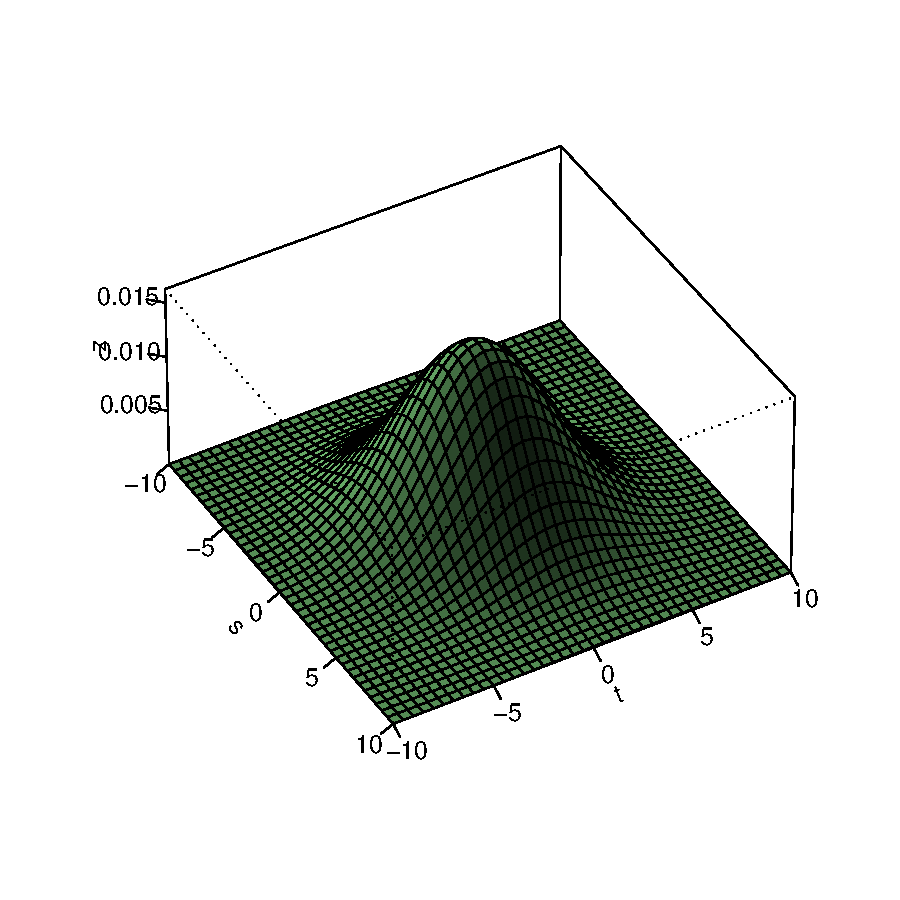
\includegraphics[width=3.25in]{Images/Rho2.pdf}} 
\end{minipage}
\hspace{0.0in}
\begin{minipage}[b]{0.65\linewidth}
    \mbox{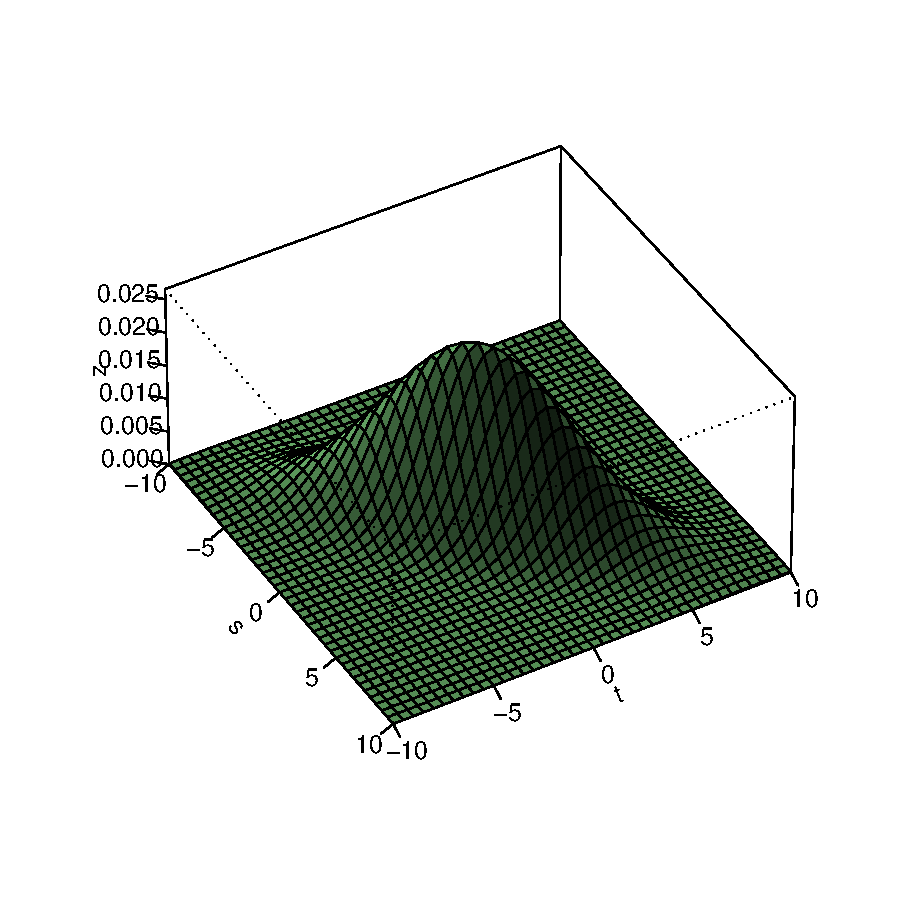
\includegraphics[width=3.25in]{Images/Rho8.pdf}} 
\end{minipage}

Let's call the two variables $X_1$ and $X_2$, with the corresponding
axes in the graphs to be referred to as $t_1$ and $t_2$.  The first
graph was generated with a correlation of 0.2 between the two variables,
while in the second one, the correlation is 0.8.

Not surprisingly due to the high correlation in the second graph, the
``two-dimensional bell'' is concentrated around a straight line,
specifically the line $t_2 = - t_1$.  In other words, there is high
probability that $X_2 \approx -X_1$, so that  

\begin{quote}

To a large extent, there is only one variable here, $X_1$ (or other
choices, e.g.\ $X_2$), not two.  

\end{quote}

Note one more time, though, the approximate nature of the approach we
are developing.  There really \textit{are} two variables above.  By
using only one of them, we are relinquishing some information.  But with
the need to avoid overfitting, use of the approximation may be a net win
for us.

\subsubsection{Eigenanalysis}

Well then, how can we determine a set of near-redundant variables, so
that we can consider omitting them from our analysis?  Let's look at
those graphs a little more closely.

Any \textit{level set} in the above graphs, i.e.\ a curve one
obtains by slicing the bells parallel to the $(t_1,t_2)$ axis can be
shown to be an ellipse.  As noted, the major axis of the ellipse will be
the line $t_1 + t_2 = 0$.  The minor axis will be the line perpendicular
to that, $t_1 - t_2 = 0$.  In turn, that means that standard probability
methods can then be used to show that the variables

\begin{equation}
Y_1 = X_1 + X_2 
\end{equation}

and 

\begin{equation}
Y_2 = X_1 - X_2 
\end{equation}

have 0 correlation.  Then we have a good case for using only $Y_1$ in
our data analysis, instead of using $X_1$ and $X_2$.  

But why not use just $X_1$?  As usual in statistics/ML, things get more
complicated in higher dimensions.  In choosing variables to retain in
our analysis, it makes sense to require that they be uncorrelated, as
$Y_1$ and $Y_2$ are above; if not, intuitively there is some redundancy
among them, which of course is what we are hoping to avoid.  

With that in mind, now suppose we have $p$ variables, $X_1,
X_2,...,X_p$, not just two.  We can no longer visualize in higher
dimensions, but one can show that the level sets will be be
$p$-dimensional ellipsoids.  These now have $p$ axes rather than just
two, and we can define $p$ new variables, $Y_1,Y_2,...,Y_p$ from the
$X_i$, such that:

\begin{itemize}

\item [(a)] The $Y_i$ are uncorrelated.

\item [(b)] We can order them in terms of variance:

\begin{equation}
Var(Y_1) > Var(Y_2) > ... > Var(Y_p)
\end{equation}

\end{itemize} 

Now we have a promising solution to our dimension reduction problem.
In [(b)] above, we can choose to use just the first few of the $Y_i$,
omitting the ones with small variance.

That's of central importance.  In attempting dimension reduction, 

For reasons to be explained later, we'll start with square matrices, say
$G$, and in fact impose another condition, that $G$ is
\textit{symmetric}:

\begin{equation}
G' = G
\end{equation}

where $'$ denotes matrix transpose.  


Recall that for any square matrix $L$, if there is a scalar $\lambda$
and a nonzero vector $x$ such that 

\begin{equation}
Lx = \lambda x
\end{equation}

then we say that $x$ is an \textit{eigenvector} of $L$, with
\textit{eigenvalue} $\lambda$.
